\documentclass[conference]{IEEEtran}
\usepackage{cite}
\usepackage{amsmath,amssymb,amsfonts}
\usepackage{graphicx}
\usepackage{textcomp}
\usepackage{xcolor}
\usepackage{listings}
\usepackage{url}
\usepackage{hyperref}
\usepackage{tikz}
\usepackage{booktabs}
\usetikzlibrary{shapes.geometric, arrows.meta, positioning, fit, backgrounds}

\lstset{
  basicstyle=\ttfamily\scriptsize,
  breaklines=true,
  frame=single,
  language=Python,
  keywordstyle=\color{blue},
  commentstyle=\color{gray},
  stringstyle=\color{red},
  showstringspaces=false,
  numbers=left,
  numberstyle=\tiny\color{gray},
  xleftmargin=2em,
  framexleftmargin=1.5em
}

\def\BibTeX{{\rm B\kern-.05em{\sc i\kern-.025em b}\kern-.08em
    T\kern-.1667em\lower.7ex\hbox{E}\kern-.125emX}}

\begin{document}

\title{Rakshan: A Secure QR-Based Event Ticketing Platform on AWS Cloud}

\author{\IEEEauthorblockN{Tarun Chintakunta}
\IEEEauthorblockA{Student ID: x25180754 \\
MSc in Cloud Computing \\
National College of Ireland \\
Dublin, Ireland \\
x25180754@student.ncirl.ie}}

\maketitle

\begin{abstract}
This paper presents Rakshan, a cloud-native event ticketing platform that employs cryptographically signed QR codes for secure ticket generation and validation. The system addresses the prevalent issue of ticket fraud in event management by implementing HMAC-SHA256 digital signatures embedded within QR codes, ensuring ticket authenticity through a two-layer verification mechanism. The application is architected as a full-stack web platform deployed entirely on Amazon Web Services, leveraging six distinct cloud services: DynamoDB for NoSQL data persistence, S3 for static asset hosting and QR code storage, Lambda for serverless ticket processing, Elastic Beanstalk for application deployment, Cognito for identity verification, and IAM for access control. A custom Python library, \texttt{qr\_ticket\_manager}, was developed to encapsulate the cryptographic ticket lifecycle, including generation, QR encoding, and multi-layer validation. The platform demonstrates the practical application of cloud architectural patterns including serverless computing, managed NoSQL databases, and infrastructure-as-code deployment, while maintaining security through JWT authentication, bcrypt password hashing, and HMAC-based ticket integrity verification.
\end{abstract}

\section{Introduction}

Event management systems face a persistent challenge with ticket fraud, counterfeiting, and unauthorized duplication. Traditional ticketing approaches that rely on sequential numbering or simple barcodes are vulnerable to reproduction, resulting in revenue losses and logistical complications at venue entry points \cite{nair2019}. The emergence of cloud computing has provided new opportunities to build scalable, secure ticketing solutions that leverage distributed infrastructure and managed services to address these challenges effectively \cite{mell2011}. Modern cloud platforms offer serverless computing, managed databases, and identity services that significantly reduce the engineering burden of building production-grade applications while improving security posture and operational resilience \cite{jonas2019}.

This project presents Rakshan, a cloud-based event ticketing platform designed to eliminate ticket fraud through cryptographic signing of QR-coded tickets. The name ``Rakshan'' derives from the Sanskrit word for ``protection,'' reflecting the system's core objective of safeguarding event access through tamper-proof digital tickets. The platform was developed to fulfil the requirements of the Cloud Platform Programming module, demonstrating the practical integration of multiple Amazon Web Services into a cohesive, production-grade application.

The primary objectives of this project are threefold. First, to design and implement a custom Python library that provides HMAC-SHA256 based ticket generation and two-layer validation, serving as a reusable component for any QR-based authentication system. Second, to architect a full-stack application that programmatically integrates at least five AWS cloud services, applying cloud-native design patterns such as serverless computing and managed databases. Third, to deploy a publicly accessible application that demonstrates end-to-end functionality from user registration through ticket generation to real-time QR code scanning and validation at event entry points.

The remainder of this paper is structured as follows. Section II defines the functional and non-functional requirements. Section III presents the system architecture and design decisions. Section IV describes the custom library. Section V analyses the cloud services employed. Section VI documents the implementation details. Section VII covers deployment and continuous delivery. Section VIII concludes with findings and reflections.

\section{Project Specification and Requirements}

\subsection{Functional Requirements}

The application implements a comprehensive set of functional requirements spanning user management, event administration, and ticket lifecycle operations. Users can register accounts with email verification through Amazon Cognito, ensuring only legitimate email addresses are associated with accounts. The registration process triggers a six-digit one-time password sent to the user's email, which must be confirmed before full access is granted. Authenticated users can browse published events, view event details including capacity, date, location, and description information, and register for events subject to capacity constraints that are enforced through real-time DynamoDB queries.

Upon successful event registration, the system automatically invokes an AWS Lambda function that generates a cryptographically signed ticket with an embedded QR code. The QR code image is stored in Amazon S3 for retrieval, and the ticket record is persisted in DynamoDB with a reference to the QR asset. Users can view their tickets and associated QR codes through a dedicated ``My Tickets'' interface. At event venues, administrators can scan QR codes using the built-in scanner page to validate ticket authenticity through a two-layer verification process that checks both the HMAC-SHA256 signature and the ticket status in the database, preventing both forgery and reuse of already-scanned tickets.

Administrators have access to a dashboard providing event analytics including total registrations, check-in counts, and revenue metrics. The admin interface supports attendee management with a detailed list of registered users per event and CSV export functionality for offline record keeping. The system enforces complete CRUD operations across events, registrations, and tickets, with role-based access controls distinguishing between regular users and administrators through JWT token claims.

\subsection{Non-Functional Requirements}

The platform addresses several non-functional requirements critical to a production ticketing system. Security is enforced through multiple layers: JWT tokens for session management with configurable 24-hour expiration, bcrypt hashing with automatic salt generation for password storage, HMAC-SHA256 signatures for ticket integrity, and CORS configuration restricting API access to authorised origins. Scalability is achieved through DynamoDB, which provides consistent single-digit millisecond performance at any scale through automatic partitioning, and Lambda functions that scale automatically with demand without requiring server provisioning \cite{aws2024dynamodb}. Availability is supported by Elastic Beanstalk with health monitoring and automatic instance recovery. The system maintains responsiveness through a single-page application architecture with optimistic UI updates, loading states, and error boundaries. Data consistency is maintained through DynamoDB's strongly consistent reads for critical operations such as ticket validation and capacity checking, preventing race conditions during high-demand registration periods.

\section{Architecture and Design}

\subsection{System Architecture}

The application follows a three-tier architecture pattern adapted for cloud deployment, combining traditional client-server patterns with serverless components to optimise for both development velocity and operational scalability. The presentation tier is a React single-page application hosted on Amazon S3 as a static website, eliminating the need for a dedicated web server. The application tier is a Flask REST API deployed on AWS Elastic Beanstalk, providing managed compute with automatic health monitoring. The data tier uses Amazon DynamoDB as the primary datastore with S3 serving as the object store for binary assets. Serverless compute via AWS Lambda handles the computationally intensive ticket generation and validation operations, decoupling these from the synchronous request-response cycle of the Flask API.

\begin{figure}[htbp]
\centerline{
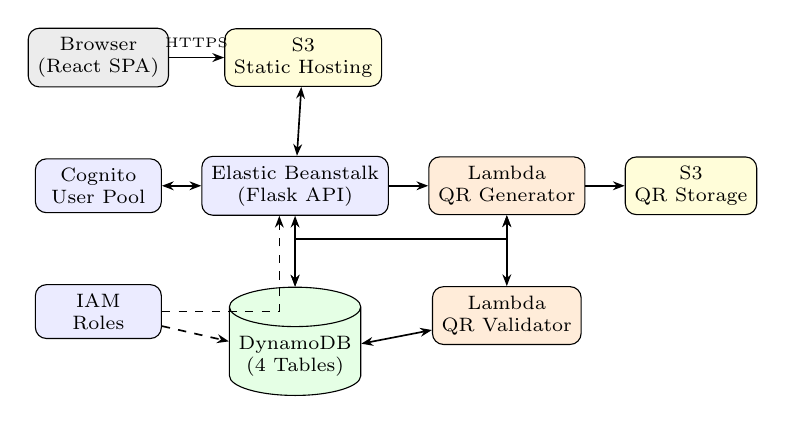
\begin{tikzpicture}[
    node distance=0.6cm and 0.5cm,
    every node/.style={font=\scriptsize},
    service/.style={rectangle, draw, rounded corners, minimum width=1.6cm, minimum height=0.65cm, align=center, fill=blue!8},
    lambda/.style={rectangle, draw, rounded corners, minimum width=1.6cm, minimum height=0.65cm, align=center, fill=orange!15},
    db/.style={cylinder, draw, shape border rotate=90, minimum width=1.3cm, minimum height=0.65cm, align=center, fill=green!10, aspect=0.3},
    storage/.style={rectangle, draw, rounded corners, minimum width=1.6cm, minimum height=0.65cm, align=center, fill=yellow!15},
    client/.style={rectangle, draw, rounded corners, minimum width=1.6cm, minimum height=0.65cm, align=center, fill=gray!15},
    arr/.style={-{Stealth[length=1.5mm]}, semithick},
    darr/.style={{Stealth[length=1.5mm]}-{Stealth[length=1.5mm]}, semithick}
]

% Row 1: Client -> S3 Frontend
\node[client] (browser) {Browser\\(React SPA)};
\node[storage, right=0.7cm of browser] (s3fe) {S3\\Static Hosting};

% Row 2: Cognito | EB | Lambda Gen | S3 QR
\node[service, below=0.9cm of browser] (cognito) {Cognito\\User Pool};
\node[service, right=0.5cm of cognito] (eb) {Elastic Beanstalk\\(Flask API)};
\node[lambda, right=0.5cm of eb] (lamgen) {Lambda\\QR Generator};
\node[storage, right=0.5cm of lamgen] (s3qr) {S3\\QR Storage};

% Row 3: IAM | DynamoDB | Lambda Val
\node[service, below=0.9cm of cognito] (iam) {IAM\\Roles};
\node[db, below=0.9cm of eb] (dynamo) {DynamoDB\\(4 Tables)};
\node[lambda, below=0.9cm of lamgen] (lamval) {Lambda\\QR Validator};

% Arrows
\draw[arr] (browser) -- node[above, font=\tiny] {HTTPS} (s3fe);
\draw[darr] (s3fe) -- (eb);
\draw[darr] (eb) -- (cognito);
\draw[darr] (eb) -- (dynamo);
\draw[arr] (eb) -- (lamgen);
\draw[arr] (lamgen) -- (s3qr);
\draw[darr] (lamgen) -- (lamval);
\draw[darr] (lamval) -- (dynamo);
\draw[darr] (lamgen) |- ([yshift=-0.3cm]lamgen.south) -| (dynamo);
\draw[arr, dashed] (iam) -- (dynamo);
\draw[arr, dashed] (iam) -| ([xshift=-0.2cm]eb.south);

\end{tikzpicture}
}
\caption{Rakshan system architecture showing six AWS cloud services and their interactions.}
\label{fig:architecture}
\end{figure}

Fig.~\ref{fig:architecture} illustrates the complete system architecture. The React frontend is served from S3 and communicates with the Flask API via RESTful HTTP requests. When a user registers for an event, the API invokes the QR Generator Lambda function, which uses the custom \texttt{qr\_ticket\_manager} library to create a signed ticket, generate a QR code image, store the image in the QR Storage S3 bucket, and persist the ticket record in DynamoDB. During event check-in, the QR Validator Lambda is invoked with the scanned QR data, performs signature verification and status checking against DynamoDB, and marks the ticket as used to prevent re-entry. IAM roles govern the permissions between all services, enforcing the principle of least privilege throughout the architecture.

\subsection{Database Design}

DynamoDB was selected over relational alternatives due to its serverless operational model, predictable performance at scale, and native integration with other AWS services \cite{aws2024dynamodb}. The data model consists of four tables, each designed around specific access patterns identified during requirements analysis. Table~\ref{tab:dynamodb} summarises the schema design.

\begin{table}[htbp]
\caption{DynamoDB Table Design}
\label{tab:dynamodb}
\centering
\begin{tabular}{@{}llll@{}}
\toprule
\textbf{Table} & \textbf{Partition Key} & \textbf{GSI(s)} \\
\midrule
Users & user\_id & email \\
Events & event\_id & status \\
Registrations & registration\_id & user\_id, event\_id \\
Tickets & ticket\_id & registration\_id \\
\bottomrule
\end{tabular}
\end{table}

The Users table stores account information with \texttt{user\_id} as the partition key and a Global Secondary Index on the \texttt{email} attribute, enabling efficient lookup during login without scanning the entire table. The Events table uses a GSI on \texttt{status} to retrieve only active events for the public listing page. The Registrations table maintains two GSIs: one on \texttt{user\_id} for the ``My Tickets'' page and one on \texttt{event\_id} for administrator attendee listings. The Tickets table uses a GSI on \texttt{registration\_id} to link tickets back to their originating registration, supporting the one-to-one relationship between registrations and tickets. This single-table-per-entity approach was chosen over a single-table design for clarity and maintainability, accepting some additional read cost for cross-entity queries in exchange for a more intuitive data model suitable for the project's scale \cite{dynamodbbook2020}.

\subsection{Security Architecture}

The security model implements defence in depth across multiple layers, following AWS security best practices \cite{awsiam2024}. At the network layer, the API is accessible only through the Elastic Beanstalk load balancer endpoint. At the authentication layer, JSON Web Tokens signed with a server-side secret carry user identity and role claims, with tokens validated on every protected request through a custom \texttt{token\_required} middleware decorator. At the data layer, passwords are hashed using bcrypt with automatic salt generation, preventing rainbow table and brute-force attacks. At the identity layer, Amazon Cognito enforces email verification through OTP codes before accounts receive full access. At the ticket integrity layer, HMAC-SHA256 signatures computed over the ticket payload using a dedicated secret key make it computationally infeasible to forge valid tickets without knowledge of the signing key. The two-layer validation approach at check-in first verifies the cryptographic signature and then checks the ticket status in DynamoDB, preventing both forgery and replay attacks where a valid ticket QR code might be photographed and reused.

\section{Library Description}

\subsection{Purpose and Rationale}

The \texttt{qr\_ticket\_manager} library was developed as a standalone Python package to encapsulate the complete ticket lifecycle: generation, QR code creation, and validation. The decision to implement this as a separate library rather than inline application code was motivated by several factors. The same cryptographic logic is required in both Lambda functions (generator and validator) and potentially in the Flask API, making code reuse essential for consistency and maintainability. Publishing the library as an installable package with \texttt{setup.py} and \texttt{pyproject.toml} enables independent versioning, testing with pytest, and potential reuse in other projects requiring QR-based authentication. The library follows object-oriented design principles, with each class encapsulating a distinct responsibility and a custom exception hierarchy providing granular error handling.

The library is available at: \url{https://github.com/Tarunchintakunta/CPPRak} within the \texttt{qr\_ticket\_manager/} directory, installable via \texttt{pip install -e .} from the package root.

\subsection{Library Structure and Implementation}

The library comprises four core classes and eight custom exception types. The \texttt{TicketGenerator} class handles UUID-based ticket ID generation and HMAC-SHA256 payload signing, producing a deterministic signature over a JSON-serialised payload with sorted keys to ensure signature consistency regardless of dictionary insertion order. The \texttt{QRCodeCreator} class generates QR code images using the \texttt{qrcode} library with high error correction (level H, supporting up to 30\% damage tolerance), producing PNG images suitable for both digital display and physical printing. The \texttt{TicketValidator} class performs the two-layer ticket verification, accepting an optional database callback function for status lookups that decouples the validation logic from any specific persistence layer. The \texttt{TicketLogger} class provides structured logging with contextual fields across all operations.

\begin{lstlisting}[caption={HMAC-SHA256 ticket generation in TicketGenerator.}, label={lst:generator}]
class TicketGenerator:
    def __init__(self, secret_key: str):
        if not secret_key:
            raise TicketGenerationError(
                "Secret key must not be empty")
        self.secret_key = secret_key

    def create_signature(self, payload: dict):
        payload_str = json.dumps(
            payload, sort_keys=True, default=str)
        return hmac.new(
            self.secret_key.encode("utf-8"),
            payload_str.encode("utf-8"),
            hashlib.sha256).hexdigest()

    def generate_ticket(self, event_id,
            registration_id, user_id, event_name):
        ticket_id = str(uuid.uuid4())
        payload = {
            "ticket_id": ticket_id,
            "event_id": event_id,
            "registration_id": registration_id,
            "user_id": user_id,
            "event_name": event_name,
            "created_at": datetime.now(
                timezone.utc).isoformat(),
        }
        signature = self.create_signature(payload)
        return {"ticket_id": ticket_id,
            "payload": payload,
            "signature": signature,
            "status": "valid"}
\end{lstlisting}

The \texttt{TicketValidator} class implements the two-layer validation mechanism as shown in Listing~\ref{lst:validator}. Layer one performs cryptographic verification by recomputing the HMAC-SHA256 signature from the embedded payload and comparing it against the signature carried in the QR code data. Any modification to the payload fields, including the ticket ID, event reference, or timestamp, results in a signature mismatch and immediate rejection. Layer two checks the ticket status against the database to prevent reuse of already-scanned tickets, revoked tickets, or expired tickets, each raising a distinct exception type for precise error reporting at the scanner interface.

\begin{lstlisting}[caption={Two-layer validation in TicketValidator.}, label={lst:validator}]
class TicketValidator:
    VALID_STATUSES = {
        "valid", "used", "revoked", "expired"}

    def validate_ticket(self, qr_data,
            get_ticket_status=None):
        data = json.loads(qr_data)
        ticket_id = data.get("ticket_id")
        payload = data.get("payload")
        signature = data.get("signature")
        # Layer 1: Cryptographic verification
        self.verify_signature(payload, signature)
        # Layer 2: Database status check
        if get_ticket_status:
            status = get_ticket_status(ticket_id)
        else:
            status = "valid"
        self.check_status(status)
        return {"valid": True,
            "ticket_id": ticket_id,
            "event_id": payload.get("event_id"),
            "message": "Ticket is valid"}
\end{lstlisting}

The library includes 15 unit tests covering signature generation correctness, validation success paths, all failure modes (invalid signature, already used, revoked, expired), QR code image creation, and error handling for malformed inputs.

\section{Cloud Services Analysis}

This section critically analyses each of the six AWS cloud services integrated into the application, providing justification for their selection over alternatives.

\subsection{Amazon DynamoDB}

DynamoDB serves as the sole database for all application data across four tables. The choice of DynamoDB over Amazon RDS or Aurora was driven by several factors. DynamoDB's serverless model eliminates database administration overhead including patching, backup scheduling, and capacity planning, as on-demand billing scales automatically with workload \cite{aws2024dynamodb}. The key-value access patterns in this application, where entities are primarily retrieved by their primary key or through well-defined secondary indices, align naturally with DynamoDB's data model. The trade-off is the loss of complex query flexibility offered by SQL databases, particularly for ad-hoc analytical queries; however, the application's access patterns were designed upfront to work within DynamoDB's constraints, using GSIs for the required query dimensions. DynamoDB's integration with Lambda through the AWS SDK enables direct read and write operations from serverless functions without the connection pooling concerns that commonly affect relational databases in serverless contexts, where the ephemeral nature of Lambda execution environments can exhaust connection limits \cite{awslambdadynamo2023}.

\subsection{Amazon S3}

S3 is used for two distinct purposes within the architecture. First, the React frontend is hosted as a static website on S3 with the \texttt{index.html} configured as both the index and error document, enabling client-side routing for the single-page application. S3 static website hosting provides high availability through automatic replication across multiple Availability Zones at minimal cost compared to running a dedicated web server on EC2 or ECS \cite{awss3hosting2024}. Second, a separate S3 bucket (\texttt{rakshan-qr-tickets}) stores generated QR code images, which are referenced by their S3 key in ticket records and served through the Flask API's ticket endpoint. This separation of binary assets from the database follows the recommended pattern for DynamoDB, which is optimised for items under 400 KB rather than binary large objects. An alternative approach of storing base64-encoded images directly in DynamoDB was considered but rejected due to the increased item size and read capacity consumption.

\subsection{AWS Lambda}

Two Lambda functions handle the ticket processing operations that are central to the application's value proposition. The QR Generator Lambda is invoked synchronously when a user registers for an event. It accepts the event, registration, and user identifiers, generates the signed ticket using the \texttt{qr\_ticket\_manager} library, creates a QR code image, uploads it to S3, and writes the ticket record to DynamoDB. Listing~\ref{lst:lambda} demonstrates this integration.

\begin{lstlisting}[caption={Lambda QR Generator using the custom library.}, label={lst:lambda}]
from qr_ticket_manager import (
    TicketGenerator, QRCodeCreator)

def handler(event, context):
    config = _get_config(event)
    generator = TicketGenerator(
        config["secret_key"])
    ticket = generator.generate_ticket(
        event_id, registration_id,
        user_id, event_name)
    qr_payload = generator.create_qr_payload(
        ticket)
    qr_creator = QRCodeCreator()
    image_bytes = qr_creator.generate_qr_image(
        qr_payload)
    # Store QR image in S3
    s3_client.put_object(
        Bucket=config["s3_bucket"],
        Key=f"qr_codes/{ticket['ticket_id']}.png",
        Body=image_bytes,
        ContentType="image/png")
    # Persist ticket record in DynamoDB
    table.put_item(Item={
        "ticket_id": ticket["ticket_id"],
        "status": ticket["status"],
        "signature": ticket["signature"]})
\end{lstlisting}

The QR Validator Lambda processes scanned QR codes during event check-in, performing signature verification, status lookup in DynamoDB, and marking validated tickets as used. Lambda was selected over processing these operations within the Flask API for two reasons. First, Lambda's automatic scaling ensures ticket generation remains responsive even during peak registration periods without requiring horizontal scaling of the Flask application \cite{awslambda2024}. Second, isolating the cryptographic operations in Lambda functions provides a security boundary, as the ticket signing secret key is configured only in the Lambda environment variables rather than the web application server, reducing the attack surface for key compromise.

\subsection{AWS Elastic Beanstalk}

Elastic Beanstalk manages the deployment and lifecycle of the Flask API, abstracting infrastructure provisioning while retaining full configuration control through \texttt{.ebextensions}. The platform provides automatic health monitoring, log aggregation, and rolling deployments through versioned application bundles. Compared to deploying directly on EC2, Elastic Beanstalk reduces operational complexity by managing load balancing, security group configuration, and application process management through Gunicorn \cite{awseb2024}. Compared to containerised alternatives such as ECS or EKS, Elastic Beanstalk was selected for its simpler deployment model appropriate for a single-service API. The overhead of Dockerfiles, container registries, and orchestration manifests was unjustified given that the application consists of a single Python service with straightforward dependency management.

\subsection{Amazon Cognito}

Cognito provides managed email verification during user registration, handling the complete OTP lifecycle including code generation, email delivery, expiration management, and rate limiting. The application integrates with Cognito's User Pool through the \texttt{boto3} SDK, calling \texttt{sign\_up} during registration, \texttt{confirm\_sign\_up} for code verification, and \texttt{resend\_confirmation\_code} for code re-delivery. Cognito was chosen over implementing custom email verification using Amazon SES because Cognito provides a unified solution that eliminates the need to build and maintain email templates, delivery retry logic, code storage, and expiration handling \cite{awscognito2024}. The integration is environment-aware through the configuration hierarchy: \texttt{USE\_COGNITO} is set to \texttt{False} in \texttt{DevelopmentConfig} and \texttt{True} in \texttt{ProductionConfig}, ensuring local development does not depend on external AWS services.

\subsection{AWS IAM}

IAM governs all inter-service permissions through the principle of least privilege. The Elastic Beanstalk EC2 instance role (\texttt{aws-elasticbeanstalk-ec2-role}) is configured with managed policies granting \texttt{AmazonDynamoDBFullAccess}, \texttt{AmazonS3FullAccess}, \texttt{AWSLambda\_FullAccess}, and Cognito access, enabling the Flask API to interact with all dependent services. Each Lambda function has its own execution role with policies scoped to the specific DynamoDB tables and S3 buckets it requires. While the current implementation uses AWS managed policies for development velocity, a production hardening step would replace these with custom policies specifying resource ARNs and action subsets to further constrain permissions \cite{awsiam2024}.

\section{Implementation}

\subsection{Backend API Implementation}

The Flask backend is structured as a Python package using the application factory pattern, with five route blueprints registered during initialisation. The authentication blueprint (\texttt{/api/auth/}) implements five endpoints: \texttt{POST /register} for account creation with Cognito sign-up, \texttt{POST /verify-email} for OTP confirmation, \texttt{POST /resend-code} for code re-delivery, \texttt{POST /login} for JWT token issuance, and \texttt{GET /me} for profile retrieval. The events blueprint (\texttt{/api/events/}) provides full CRUD with admin-only write access enforced through a custom \texttt{@token\_required} decorator. The registrations blueprint handles capacity-checked event registration with automatic Lambda invocation for ticket generation. The tickets blueprint serves ticket details and QR code images retrieved from S3. The admin blueprint provides dashboard aggregation queries across all four DynamoDB tables and CSV export through dynamic report generation.

\subsection{Frontend Application}

The frontend is implemented as a React 19 single-page application with Vite as the build tool and Tailwind CSS v4 for utility-first styling. The application implements ten distinct pages covering the complete user journey: a landing page, authentication pages (login, register, email verification), event browsing and detail pages, ticket management pages (listing and detail with QR code display), and three administrative pages (dashboard, event creation, QR scanner). Authentication state management uses React Context, providing \texttt{user}, \texttt{login}, \texttt{register}, \texttt{logout}, and \texttt{refreshUser} functions to all components. API communication is centralised through an Axios instance with request interceptors for JWT injection and response interceptors for automatic 401 handling that clears stored credentials and redirects to the login page.

\subsection{Cognito Email Verification Integration}

The Cognito integration required careful design to support both local development and production deployment without code duplication. The \texttt{CognitoService} class encapsulates all Cognito operations behind an \texttt{enabled} flag derived from the application configuration. When disabled, all methods return immediately with no-op behaviour, allowing the registration flow to proceed without external dependencies during local development. In production, the service creates a \texttt{boto3} Cognito Identity Provider client and exposes four operations: \texttt{sign\_up} triggers the verification email, \texttt{verify\_email} confirms the OTP code, \texttt{resend\_code} re-delivers the code, and \texttt{is\_verified} checks the user's confirmation status in the Cognito User Pool. The login endpoint includes a synchronisation mechanism that checks Cognito's verification status when the local DynamoDB record shows unverified, updating the local record if verification was completed externally, ensuring consistency between the two identity stores.

\begin{lstlisting}[caption={Cognito service with environment-aware toggling.}, label={lst:cognito}]
class CognitoService:
    def __init__(self, app_config):
        self.enabled = getattr(
            app_config, "USE_COGNITO", False)
        if self.enabled:
            self.client = boto3.client(
                "cognito-idp",
                region_name=app_config.AWS_REGION)

    def sign_up(self, email, password, name):
        if not self.enabled:
            return False
        self.client.sign_up(
            ClientId=self.client_id,
            Username=email,
            Password=password,
            UserAttributes=[
                {"Name": "email", "Value": email},
                {"Name": "name", "Value": name}])
        return True

    def verify_email(self, email, code):
        if not self.enabled:
            return True
        self.client.confirm_sign_up(
            ClientId=self.client_id,
            Username=email,
            ConfirmationCode=code)
        return True
\end{lstlisting}

\subsection{Ticket Lifecycle}

The complete ticket lifecycle spans registration through validation. When a user clicks ``Register'' on an event page, the frontend sends a POST request to \texttt{/api/registrations/}. The backend validates event capacity through a DynamoDB query counting active registrations, checks for duplicate registrations using the \texttt{user\_id}-\texttt{event\_id} GSI, creates the registration record, and invokes the QR Generator Lambda synchronously. The Lambda function uses \texttt{TicketGenerator} to produce a signed ticket, \texttt{QRCodeCreator} to render the QR image, uploads the image to S3, writes the ticket to DynamoDB, and returns the ticket ID and QR URL. The user can then view their ticket with the embedded QR code. At the event, an administrator scans the QR code, triggering the Validator Lambda which recomputes the HMAC signature, verifies it matches, checks the DynamoDB status is ``valid'', marks the ticket as ``used'' with a timestamp, and returns a success response displayed on the scanner interface.

\section{Deployment and Continuous Delivery}

The application uses Git for version control with a private GitHub repository (\url{https://github.com/Tarunchintakunta/CPPRak}). The deployment process follows a structured workflow. The React frontend is built with the production API URL injected through the \texttt{VITE\_API\_URL} environment variable during the Vite build step, and the resulting static assets are synchronised to the S3 hosting bucket using the AWS CLI \texttt{s3 sync} command with the \texttt{--delete} flag to remove stale assets.

The backend deployment uses Elastic Beanstalk's application versioning system. The Flask application directory is packaged as a ZIP file and uploaded to the EB-managed S3 bucket, then a new application version is created and deployed to the \texttt{rakshan-prod} environment. Environment-specific configuration is managed through the \texttt{.ebextensions/01\_flask.config} file, which sets environment variables including \texttt{FLASK\_ENV}, \texttt{TICKET\_SECRET\_KEY}, \texttt{S3\_BUCKET}, \texttt{AWS\_REGION}, \texttt{COGNITO\_USER\_POOL\_ID}, and \texttt{COGNITO\_CLIENT\_ID}. The \texttt{Procfile} specifies the Gunicorn WSGI server binding to port 8000 as required by the EB platform.

Lambda functions are deployed as ZIP packages containing both the handler code and the \texttt{qr\_ticket\_manager} library with all dependencies. A notable deployment challenge arose from cross-platform binary compatibility: the Pillow imaging library, required for QR code generation, ships platform-specific compiled extensions. Development on macOS ARM required explicit targeting of \texttt{manylinux\_2\_28\_x86\_64} wheel packages during dependency installation to ensure compatibility with the Lambda execution environment.

The deployed application is accessible at: \url{http://rakshan-frontend.s3-website-ap-southeast-2.amazonaws.com}

\section{Conclusions}

This project demonstrated the design, implementation, and deployment of a cloud-native event ticketing platform integrating six AWS services into a cohesive production application. Several significant findings emerged from this process that provide insight into both the capabilities and challenges of cloud-native application development.

The design of the \texttt{qr\_ticket\_manager} library reinforced the importance of separating security-critical logic into independently testable, reusable components. The HMAC-SHA256 approach provided a practical balance between cryptographic strength and implementation complexity, enabling tamper-proof tickets without the overhead of public-key infrastructure. The two-layer validation pattern, combining cryptographic and database-backed checks, effectively addresses both forgery and replay attack vectors that are common in ticketing systems.

DynamoDB's schema design required careful upfront planning of access patterns and GSI configuration, contrasting sharply with the ad-hoc query flexibility of relational databases. However, this constraint proved beneficial by forcing a disciplined data modelling approach where every query path was explicitly considered during design. The operational simplicity of a fully managed, serverless database justified this design-time investment for the project's requirements.

Lambda function deployment revealed practical challenges with cross-platform binary compatibility that are not immediately apparent during local development. The need to compile native extensions for the Linux x86\_64 Lambda runtime while developing on macOS ARM architecture required specific packaging strategies that should be automated in a CI/CD pipeline for production use.

Integrating Cognito for email verification demonstrated how managed identity services can significantly reduce the implementation burden of security-critical features. Rather than building custom email delivery, code generation, expiration logic, and rate limiting, the entire verification flow was achieved through three Cognito API calls, allowing development effort to focus on application-specific logic. The environment-aware configuration pattern, where Cognito is enabled only in production, proved essential for maintaining development velocity without external service dependencies.

Overall, the project achieved its three primary objectives: developing a functional custom library with comprehensive cryptographic ticket management, integrating six AWS cloud services programmatically into a cohesive application, and deploying a publicly accessible platform demonstrating the complete ticketing workflow from registration through QR-based event check-in.

The project could be extended in several directions for production readiness. Adding Amazon CloudFront as a CDN for both the S3-hosted frontend and S3 QR code images would improve global latency and enable HTTPS with custom domain support. Implementing infrastructure-as-code through AWS CloudFormation or Terraform would formalise the currently manual resource provisioning process. Adding a CI/CD pipeline using GitHub Actions with automated testing, building, and deployment would complete the continuous delivery workflow that is currently performed manually.

\begin{thebibliography}{00}

\bibitem{nair2019} V. Nair, R. Kumar, and S. Patel, ``QR code based event management and ticketing system,'' \textit{International Journal of Computer Applications}, vol. 178, no. 28, pp. 20--24, 2019.

\bibitem{mell2011} P. Mell and T. Grance, ``The NIST definition of cloud computing,'' \textit{National Institute of Standards and Technology}, Special Publication 800-145, 2011.

\bibitem{jonas2019} E. Jonas, J. Schleier-Smith, V. Sreekanti, C.-C. Tsai, A. Khandelwal, Q. Pu, V. Shankar, J. Carreira, K. Krauth, N. Yadwadkar, J. E. Gonzalez, R. A. Popa, I. Stoica, and D. A. Patterson, ``Cloud programming simplified: A Berkeley view on serverless computing,'' \textit{Technical Report No. UCB/EECS-2019-3}, University of California, Berkeley, 2019.

\bibitem{aws2024dynamodb} Amazon Web Services, ``Amazon DynamoDB Developer Guide,'' 2024. [Online]. Available: https://docs.aws.amazon.com/amazondynamodb/latest/developerguide/

\bibitem{dynamodbbook2020} A. DeBrie, \textit{The DynamoDB Book: Data Modeling with Amazon DynamoDB}. Self-published, 2020.

\bibitem{awslambdadynamo2023} Amazon Web Services, ``Using AWS Lambda with Amazon DynamoDB,'' 2023. [Online]. Available: https://docs.aws.amazon.com/lambda/latest/dg/with-ddb.html

\bibitem{awss3hosting2024} Amazon Web Services, ``Hosting a static website using Amazon S3,'' 2024. [Online]. Available: https://docs.aws.amazon.com/AmazonS3/latest/userguide/WebsiteHosting.html

\bibitem{awslambda2024} Amazon Web Services, ``AWS Lambda Developer Guide,'' 2024. [Online]. Available: https://docs.aws.amazon.com/lambda/latest/dg/welcome.html

\bibitem{awseb2024} Amazon Web Services, ``AWS Elastic Beanstalk Developer Guide,'' 2024. [Online]. Available: https://docs.aws.amazon.com/elasticbeanstalk/latest/dg/Welcome.html

\bibitem{awscognito2024} Amazon Web Services, ``Amazon Cognito Developer Guide,'' 2024. [Online]. Available: https://docs.aws.amazon.com/cognito/latest/developerguide/what-is-amazon-cognito.html

\bibitem{awsiam2024} Amazon Web Services, ``AWS Identity and Access Management User Guide,'' 2024. [Online]. Available: https://docs.aws.amazon.com/IAM/latest/UserGuide/introduction.html

\end{thebibliography}

\end{document}
